%!TEX encoding=UTF-8 Unicode
%!TEX root=../tabarnac.tex

\section{Design}
\label{sec:design}

\TABARNAC~ is divided in two parts: the instrumentation tool and the
visualization.  In this section we discuss the implementation of both parts.

\subsection{Implementation}
\label{sec:design-impl}

The instrumentation is done using a custom Pintool \cite{Luk05Pin}.

Before running the application, our tool retrieve static allocation
informations using the \texttt{libelfg0} library. Dynamic allocations are
intercepted using a \texttt{malloc} replacement. If the application is
compiled with the debug flags, retrieve the structure name from the source
code. If we can't retrieve a structure name, we called it
\texttt{AnonymousStruc\#ID}, where $ID$ is a unique identifier for the
execution, starting at $0$ Finally, each time a thread is created, we compute
its stack bounds, and create a virtual structures named \texttt{Stack\#N} where
$N$ is the thread id. Only structure bigger than one page are recorded as our
analysis granularity is the memory page. The data structure informations (name
size and address) are not used during the instrumentation, they are only
printed in a file at the end of the analysis to be used by the visualization
tool.

During the execution it intercept every memory access and store for each
memory pages two counters per threads: the number of reads and of writes.
\DB{Matthias maybe you can complete here}

At the end of the analysis phase we generate to file the first
\texttt{foo.full.pages.csv} contains the list of page and the number of Read
and Write per threads. And the second \texttt{foo.structs.csv} contains the
list of structures with their name, size and start address.

We then call a R-markdown script which will first read the two csv files and
retrieve the page / data structure mapping then generate the final
visualization presented in section \ref{sec:design-visu}. We use R-markdown
for the visualization as it allow us to interleave plots withs plain text
explanation and optimization hints.

\TABARNAC~ have very few dependencies and can be installed easily. If all the R
library required to generate the visualization are not present, our tool is
able to install them automatically. By default \TABARNAC~ generate the memory
trace and the visualization, but the user can also choose to only generate the
memory trace or the visualization. This is useful for people who cannot
install R on the machine used to generate the trace. Moreover it allows the
user to customize the plots generate by the R script.

\subsection{Visualization}
\label{sec:design-visu}

Providing an easy to read visualization of memory trace is a challenge. To
avoid the user the pain to deal with huge traces, we have opted for an
assisted visualization. Once the analyze phase is done, \TABARNAC~ will
generate a html page providing a summary of the trace through several plots.
This html page is generated using R markdown, which allows us to interleave
plots with explanations. Before each plot we explain how to read it, what
usual issues it can help to understand and we give hints on how to fix them.

The visualization starts with a small introduction reminding the main
principles while developing for NUMA machines, then it shows the analysis
machine's topology using hwloc\cite{Broquedis10hwloc}.

Then the visualization focuses on data structures usage. Some structures might
be ignored for two reason: either no access have been detected during the
analysis, which happens for external libraries structures, or less than one
access over ten thousands happens on them. This is done to make the output
more readable however it is possible to ask \TABARNAC~ not to ignore
structures in the second case.

The first series of plots aims at giving informations concerning the relative
importance of data structures. It shows the sizes of each data structure and the
number reed and writes done by each thread on each structure. The global
read/write patter is also displayed. These plots gives a general idea of the
structures use by threads, it allows also to identify master/slave patterns.
Moreover knowing the read/write behaviour is very useful as it determines the
possible optimization. For instance structures written only at initialization
(or very rarely) can be (relatively) easily duplicated in a way that each NUMA
node works on a local copy.
\DB{Maybe to much details here ?}

The second series of plots is probably the most important one, it show for
each thread and each structure the distribution of accesses inside the
structure. It gives an easy way to understand data sharing between threads and
structures usage. The plots presented in sections \ref{sec:exp-mat} and
\ref{sec:exp-is} comes from this section. They can be used either to
find identify inefficient memory usage or to determine the best NUMA mapping
policy.

Finally \TABARNAC~ provides a plot showing for each page of each structure
which thread was responsible for the first touch (such plot is used in section
\ref{sec:exp-ondes3d}). This information is quite relevant as the default
policy for Linux is to map a page as close as possible to the first thread
accessing it. If the first touch distribution doest not fit the actual access
distribution, the default mapping done by \emph{Linux} might not be efficient.
To improve that one can either distribute correctly the first touch or do some
manual data mapping to ensure locality of page during the execution.

\subsection{Analysis overhead}
\label{sec:expe-overhead}

\begin{figure}[htb]
    \centering
    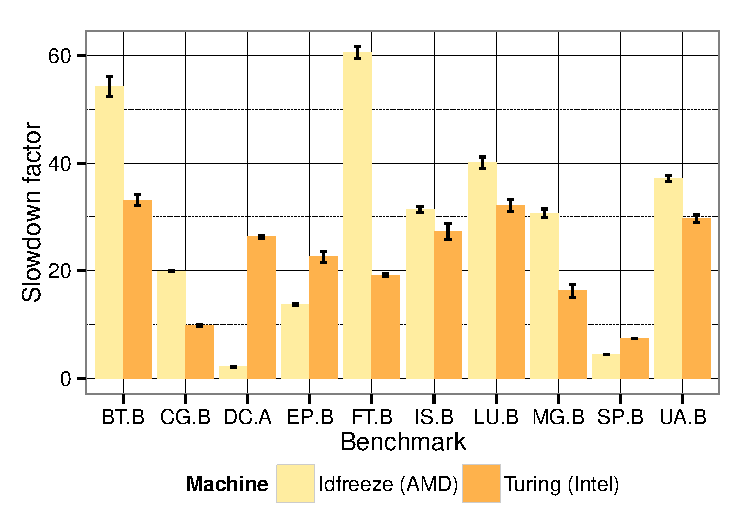
\includegraphics[width=.4\textwidth]{tool-ovh.pdf}
    \caption{Overhead of \TABARNAC~ analysis for the NAS Parallel Benchmarks.}
    \label{fig:ovh}
\end{figure}

To evaluate the analysis overhead, we ran all the NAS parallel benchmark in
class B with 64 threads on our experimental machine (see section
\ref{sec:exp-metho}) and compared the original execution time with the
execution time under instrumentation. We can see in figure \ref{fig:ovh} that
the overhead of the instrumentation is between $10$ and $30\%$. Although it is
no negligible, we have to consider the fact that often we can instrument
smaller version of the applications as we focus on the general behavior.
Moreover as we do not use sampling, our instrumentation is deterministic and
there is no need to run several times the instrumentation. Finally as our
analysis is designed to be used during the development phase of the
application and not by an automated tool during the execution, even $30\%$
overhead is quite reasonable.
